\subsection{Chapter 9 - Gravity}

\subsubsection{Overview}\label{chapter:gravity}

In previous chapters, we have so far learned about Newton's Theory of Classical Mechanics, which allowed us to model the motion of an object based on the forces acting on the object. In this chapter, we present the theories that describe the force of gravity itself. We will see several theories of gravity and focus primarily on Newton's Universal Theory of Gravity.

\begin{framed}
\textbf{Learning Objectives}\\
\begin{itemize}
\item Understand Kepler's Laws.
\item Understand Newton's Universal Theory of Gravity.
\item Understand Gauss's law and the gravitational field.
\item Understand how to use energy to describe orbits.
\item Understand how Einstein's General Theory of Relativity differs from Newton's theory of gravity.
\end{itemize}
\end{framed}

\begin{framed}
\textbf{Think About It}\\
A person stands on a scale at the top of Mount Logan, the tallest mountain in Canada. How will her measured weight compare to her weight at sea level?\}

\begin{enumerate}
\item It will be slightly less than her weight at sea level.
\item It will be equal to her weight at sea level.
\item It will be slightly more than her weight at sea level.
\end{enumerate}

\begin{framed}
\textbf{Answer}\\
\begin{enumerate}
\item
\end{enumerate}
\end{framed}
\end{framed}

\subsubsection{Kepler's Laws}

Although humans have long been fascinated by the motion of objects in the sky, it was Johannes Kepler, in the early seventeenth century, that was the first to write down quantitative rules that described the motion of planets around the Sun. His theory was based on the extensive and detailed observations recorded by Tycho Brahe in the late sixteenth century.

Kepler proposed three laws that describe all of the data that Tycho Brahe had collected about planetary motion:

\begin{enumerate}
\item The path of a planet around the Sun is described by an ellipse with the Sun at one of its foci.
\item All planets move in such a way that the area swept by a line connecting the planet and the Sun in a given period of time is constant.
\item The ratio between the orbital periods, $T$, of two planets squared is equal to the ratio of the semi-major axes, $s$, of their orbits cubed:
\end{enumerate}
\begin{equation}
\left(\frac{T_1}{T_2}\right)^2=\left(\frac{s_1}{s_2}\right)^3
\end{equation}
We examine these three laws in more detail in the sections that follow. It should also be noted that, even though Kepler's Laws were derived for planets orbiting the Sun, they apply to any body that is orbiting any other body under the influence of gravity\footnote{In fact, they apply for any two bodies orbiting each other if the force between them is an ``inverse-square'' law, such as the gravitational and electric forces.}.

\paragraph{Kepler's First Law}

Kepler noticed that the motion of all planets followed the path of an ellipse with the Sun located at one of its foci. Figure~\ref{fig:gravity:ellipse} shows a diagram of an ellipse, along with its two foci, its semi-major axis, $s$, its semi-minor axis, $b$, and its eccentricity, and the distance between a focus and the centre of the ellipse, $c$. We define the eccentricity, $e$ of the ellipse as the ratio $e=\frac{c}{s}$. The eccentricity is a measure of how far a focus is from the centre of the ellipse. A larger eccentricity thus corresponds to a ``flatter'' ellipse. Note that a circle is just a special case of an ellipse, with both foci located at the centre of the circle. The eccentriciy of a circle is thus 0.

\begin{figure}[!htbp]
\centering
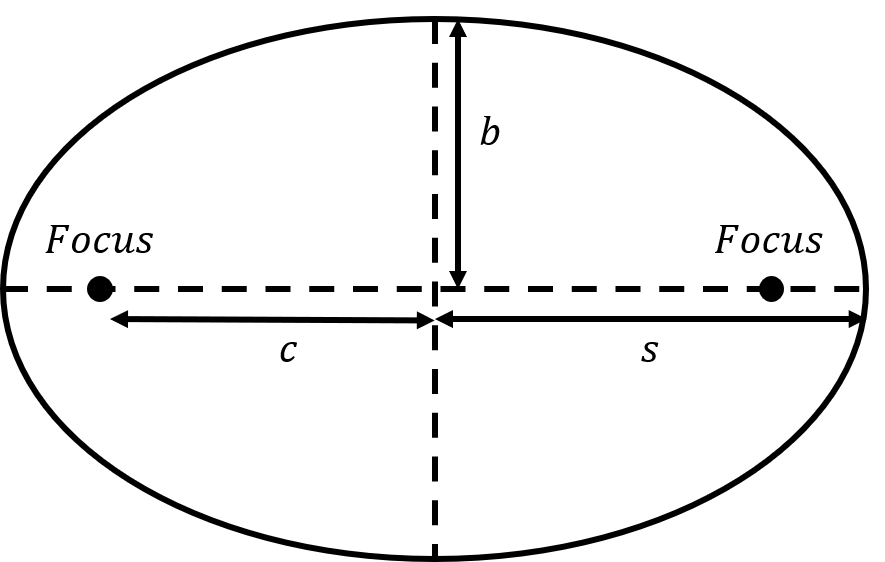
\includegraphics[width=0.5\linewidth]{files/ellipse-b667a65c43d5aca4ae37d847a50bedd1.png}
\caption[]{A ellipse, showing its two foci, its semi-major axis, $s$, its semi-minor axis, $b$, and the distance between a focus and the centre of the ellipse, $c$.}
\label{fig:gravity:ellipse}
\end{figure}

The sun is located at one of the foci. The point of closest approach to the Sun is called the ``perihelion'' of the orbit (or ``perigee'' if the orbit is around the Earth), and the point furthest from the Sun is called the ``aphelion'' of the orbit (or ``apogee'' if the orbit is around the Earth), as shown in Figure~\ref{fig:gravity:perigeeapogee}.

\begin{figure}[!htbp]
\centering
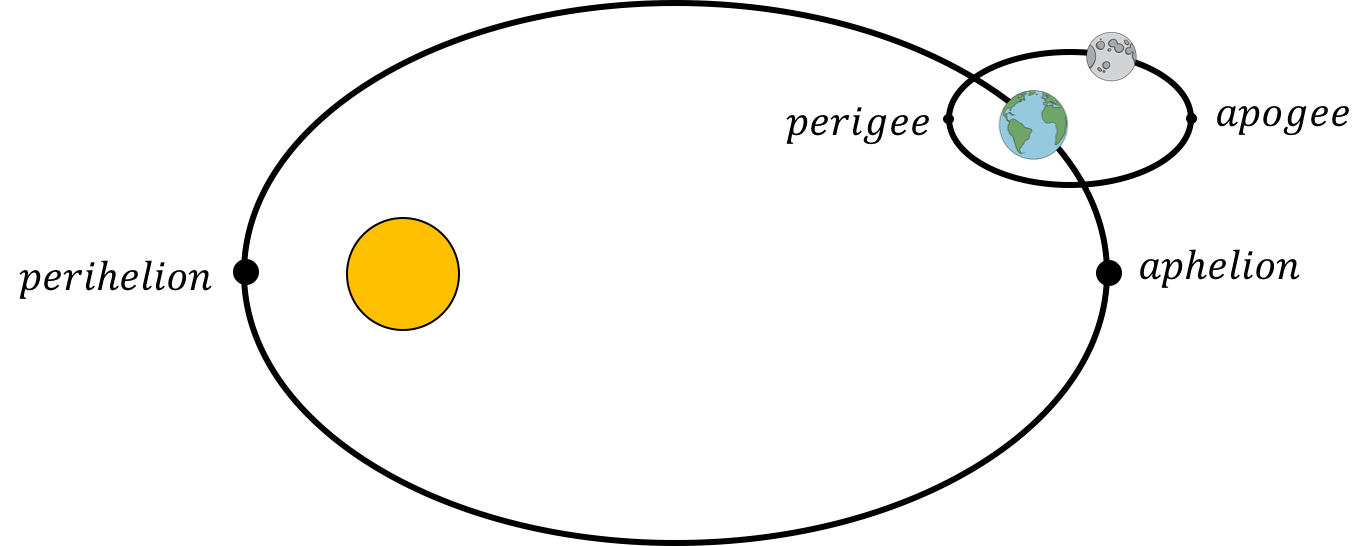
\includegraphics[width=0.7\linewidth]{files/periapogee-c6a3c9e74d40c0700ad95bdce1e3e6d3.png}
\caption[]{The orbit of the Earth around the Sun, showing the perihelion and aphelion, and the orbit of the Moon around the Earth, showing the perigee and the apogee. (Not to scale.)}
\label{fig:gravity:perigeeapogee}
\end{figure}

\begin{framed}
\textbf{Checkpoint Order the ellipses from smallest eccentricity to largest eccentricity.}\\
\begin{figure}[!htbp]
\centering
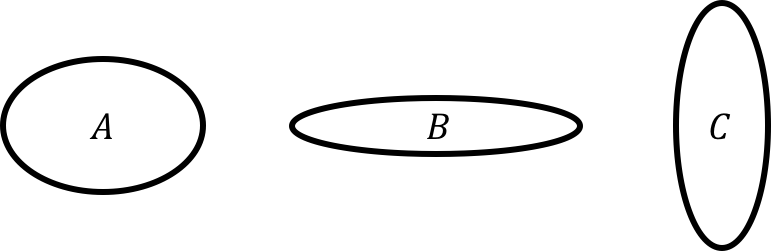
\includegraphics[width=0.7\linewidth]{files/eccellipses-23574212dfb6295ea0c1558daf1b860e.png}
\caption[]{Three ellipses, each with a different eccentricity.}
\label{fig:gravity:eccellipses}
\end{figure}

\begin{framed}
\textbf{Answer}\\
$A<C<B$
\end{framed}
\end{framed}

\paragraph{Kepler's Second Law}

Kepler's Second Law is really a statement about the speed of a planet in an elliptical orbit. It states that the area swept by a line connecting the planet and the Sun in a given period of time is fixed. This is illustrated in Figure~\ref{fig:gravity:ellipse2}, which shows the elliptical orbit of a planet around the Sun located at one of the foci, and the area swept out when the planet goes from $A$ to $B$ and from $C$ to $D$.

\begin{figure}[!htbp]
\centering
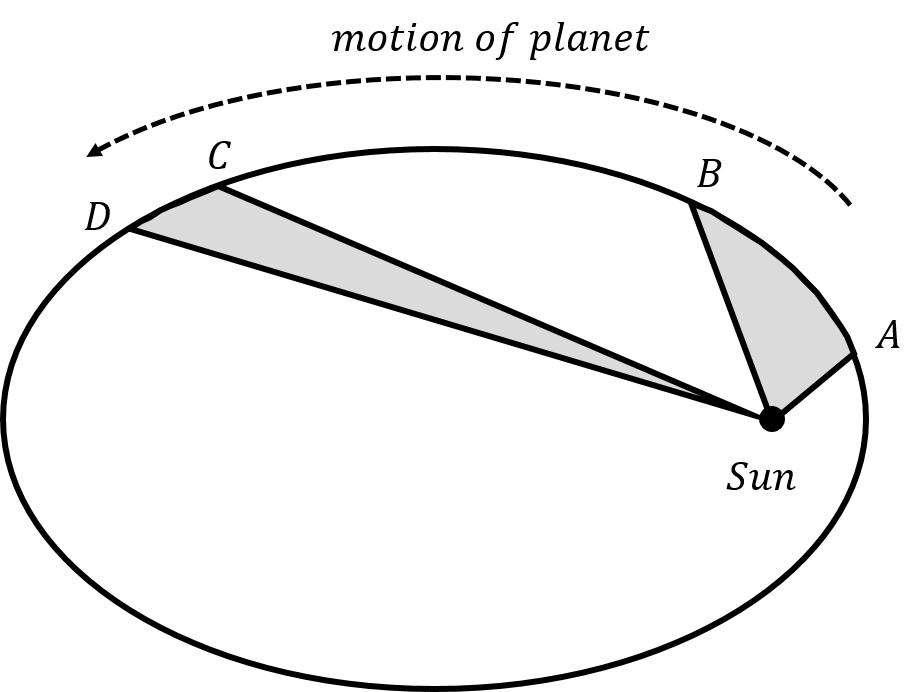
\includegraphics[width=0.45\linewidth]{files/ellipse2-0f794ab73ee184ae96b7cea9e0ddef9e.png}
\caption[]{Illustration of Kepler's Second Law, showing the area that is ``swept'' by a planet in a fixed period of time.}
\label{fig:gravity:ellipse2}
\end{figure}

Kepler's Second Law states that the two areas that are shown by the greyed out sections in the figure are the same if the planet took the same amount of time to travel between points $A$ and $B$ as it did to travel between points $C$ and $D$. Because the points $C$ and $D$ are further away from the Sun than points $A$ and $B$, the distance between points $C$ and $D$ must be smaller than the distance between points $A$ and $B$ for the two areas to be the same. This, in turn, implies that the planet must be moving slower between $C$ and $D$ than between points $A$ and $B$. The speed of a planet is thus greatest at the perihelion and smallest at the aphelion. As we will see in a later chapter, Kepler's Second Law is equivalent to the statement that the angular momentum of the planet about the Sun is conserved.

\begin{framed}
\textbf{Checkpoint}\\
Based on Kepler's second law, what can you say about the speed of a planet in a \textbf{circular} orbit?

\begin{framed}
\textbf{Answer}\\
The speed of the planet is constant.
\end{framed}
\end{framed}

\paragraph{Kepler's Third Law}

Kepler's Third Law is quantitative and relates the orbital periods ($T$) and the semi-major axes ($s$) between any two planets in orbit around the Sun:
\begin{equation}
\left(\frac{T_1}{T_2}\right)^2=\left(\frac{s_1}{s_2}\right)^3
\end{equation}
We can re-arrange this relation so that all of the quantities related to one planet are on the same side of the equal sign:
\begin{equation}
\frac{T_1^2}{s_1^3}=\frac{T_2^2}{s_2^3}=\text{constant}
\end{equation}
In other words, the ratio between the orbital period squared and the semi-major axis cubed is a constant, independent of the particular planet. In Example~9.2, we will use Newton's Universal Theory of Gravity to evaluate the constant.

\begin{framed}
\textbf{Checkpoint}\\
An object is in a circular orbit with radius $r$ and has an orbital speed $v$. If you double the radius of the circular orbit, what will be the value of the orbital speed?\}

\begin{enumerate}
\item $2v$
\item $8v$
\item $\sqrt{8}v$.
\item $\frac{1}{\sqrt{2}}v$
\end{enumerate}

\begin{framed}
\textbf{Answer}\\
\begin{enumerate}[resume]
\item
\end{enumerate}
\end{framed}
\end{framed}

\subsubsection{Newton's Universal Theory of Gravity}

Newton supposedly gained insight into the gravitational force by observing an apple falling from a tree and concluding that if it is the same force that makes apples fall at sea level and at the top of a mountain, perhaps that force can be exerted all the way up to the moon. It is rather remarkable that Newton was able to make the connection between falling apples and the motion of the moon around the Earth to find a single theory to describe both situations.

We should be clear that the theory of gravity is a different theory than Newton's ``Laws of Motion'' (Newton's Three Laws). The Laws of Motion introduce the concepts of force and inertial mass, and prescribe how to use those concepts in order to model motion using kinematics. Newton's Universal Theory of Gravity is a theory that describes the force of gravity that two bodies with (gravitational) mass exert on each other.

Newton's Universal Theory of Gravity states that if two bodies, with masses $M_1$ and $M_2$, located at positions $\vec r_1$ and $\vec r_2$, respectively, are separated by a distance, $r$, then $M_2$ will exert an attractive force on $M_1$, $\vec F_{12}$, given by:
\begin{equation}
\vec F_{12}=-G\frac{M_1M_2}{r^2}\hat r_{21}
\end{equation}
where $\hat r_{21}$ is the unit vector from $M_2$ to $M_1$:
\begin{equation}
\vec r_{21} &= \vec r_2 - \vec r_1\\
\hat r_{21} &= \frac{1}{r} \vec r_{21}
\end{equation}
as shown in Figure~\ref{fig:gravity:gvectors}. $\vec F_{12}$ should be read as ``the force on body 1 from body 2''. $G=6.67\times 10^{ -11} {\rm Nm^2/kg^2}$ is Newton's Universal Constant of Gravity. It should be noted that Newton's theory for the force of gravity written in this form only applies to either point masses (separated by a distance $r$) or spherical bodies whose centres are separated by a distance $r$ that is larger than the radius of either sphere.

\begin{figure}[!htbp]
\centering
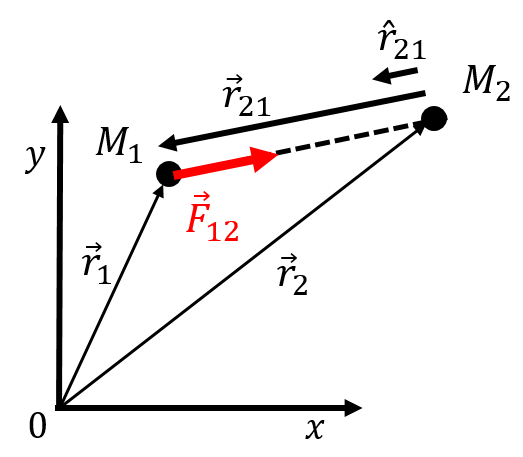
\includegraphics[width=0.4\linewidth]{files/gvectors-91e8672d8ac9e04278a36af498a9363f.png}
\caption[]{Illustration of the vectors involved in Newton's Universal Theory of Gravity.}
\label{fig:gravity:gvectors}
\end{figure}

Originally, Newton argued that the force of gravity would be proportional to the masses of the bodies, and inversely proportional to the square of the distance between them:
\begin{equation}
F_{12}\propto \frac{M_1M_2}{r^2}
\end{equation}
and $G$ is simply the constant of proportionality.

Because of Newton's Third Law, body 1 exerts a force on body 2 that is equal in magnitude but opposite in direction:
\begin{equation}
\vec F_{12} = -\vec F_{21}
\end{equation}

\begin{framed}
\textbf{Example 9.1}\\
Calculate the magnitude of the force of gravity between yourself and a person standing $50 {\rm cm}$ from you and compare that to your weight at the surface of the Earth (the force of gravity exerted by the Earth on you).\}

\begin{framed}
\textbf{Solution}\\
If we assume that the two people have a mass of $50 {\rm kg}$, the force of gravity exerted by one on the other, if they are separated by $50 {\rm cm}$, is given by:
\begin{equation}
F&=G\frac{M_1M_2}{r^2}\\
&=(6.67\times 10^{-11} {\rm Nm^2/kg^2})\frac{(50 {\rm kg})(50 {\rm kg})}{(0.5 {\rm m})^2}\\
&=6.67\times 10^{-7} {\rm N}
\end{equation}
This is a very small force, compared to their weight, $F_g$:
\begin{equation}
F_g&=M_1g\\
&=(50 {\rm kg})(9.8 {\rm N/kg})\\
&=490 {\rm N}
\end{equation}
which is approximately 700 million times bigger.

\textbf{Discussion:} The force of gravity is a very weak force when compared to other forces in Nature, such as the electric force between two charges. Newton's Universal Constant of Gravity is very small, so the force of gravity between two objects is very small unless either of the masses involved are very large, or the distance between them is very small. In general, when modelling the motion of objects on the Earth, it is generally safe to ignore the forces of gravity between objects and only include their weight (the force of gravity from the Earth).
\end{framed}
\end{framed}

\begin{framed}
\textbf{Checkpoint}\\
The radius of the Earth is 6371 \{{\textbackslash}rm km\}. What is the order of magnitude of the Earth's mass?\}

\begin{enumerate}
\item $10^{24} {\rm kg}$
\item $10^{18} {\rm kg}$
\item $10^{19} {\rm kg}$
\item $10^{21} {\rm kg}$
\item Not enough information.
\end{enumerate}

\begin{framed}
\textbf{Answer}\\
\begin{enumerate}
\item
\end{enumerate}
\end{framed}
\end{framed}

\begin{framed}
\textbf{Example 9.2}\\
Determine the constant in Kepler's Third Law for planets orbiting the Sun, namely the value of the ratio:
\begin{equation}
\frac{s^3}{T^2}
\end{equation}
where $s$ is the semi-major axis and $T$ is the orbital period.

\begin{framed}
\textbf{Solution}\\
Since Kepler's Third Law holds for any body orbiting the Sun, we can easily determine the ratio by considering a planet of mass $m$ in a circular orbit of radius $R$ centred about the Sun. The semi-major axis of the orbit is equal to the radius of the orbit for a circular orbit ($s=R$).

If the planet is in a circular orbit about the Sun, its speed, $v$, will be constant, by Kepler's Second Law, and it will thus be executing uniform circular motion. The only force exerted on the planet is the force of gravity exerted by the Sun. Thus the force of gravity must be equal to the mass of the planet times its radial (centripetal) acceleration, $a_R$, which is given by:
\begin{equation}
a_R=\frac{v^2}{R}
\end{equation}
Newton's Second Law for the planet can be written as:
\begin{equation}
\sum F = F_g &= ma_R\\
G\frac{Mm}{R^2}&=m\frac{v^2}{R}\\
G\frac{M}{R}&=v^2
\end{equation}
where $M$ is the mass of the Sun. The speed of the planet is given by the circumference of the orbit divided by the orbital period $T$, since it is constant:
\begin{equation}
v=\frac{2\pi R}{T}
\end{equation}
Re-arranging the equation from Newton's Second Law:
\begin{equation}
G\frac{M}{R}&=v^2\\
G\frac{M}{R}&=\frac{4\pi^2 R^2}{T^2}\\
\therefore \frac{R^3}{T^2}&=G\frac{M}{4\pi^2}
\end{equation}
Thus, we find that the ratio of the cube of the orbital radius to the period squared is a constant that depends only on the mass of the Sun, which will then be the same for all planets (as it does not depend on, say, the mass of the planet that we considered).

\textbf{Discussion}: The relation above can, for example, be used to determine the mass of the Sun, since we can use geometry to determine the semi-major axis for the orbit of a planet, as Kepler did with the data from Tycho Brahe.
\end{framed}
\end{framed}

\begin{framed}
\textbf{Example 9.3}\\
The acceleration due to Earth's gravity depends on the force that the Earth exerts on an object. Using the Earth's mass and radius, determine the acceleration of falling objects due to Earth's gravity at the surface of the Earth. Also, determine the altitude where the acceleration due to Earth's gravity is half of that at the Earth's surface.

\begin{framed}
\textbf{Solution}\\
We can find the acceleration due to Earth's gravity by determining the acceleration of a mass $m$ upon which gravity is the only acting force. In other words, we model an object that is in free-fall a distance $R$ away from the centre of the Earth. Newton's Second Law can be used in one dimension (corresponding to the direction that connects the falling mass to the centre of the Earth):
\begin{equation}
\sum F &= G\frac{Mm}{R^2}=ma\\
\therefore a&=G\frac{M}{R^2}
\end{equation}
where $M=5.97\times 10^{24} {\rm kg}$ is the mass of the Earth. At the surface of the Earth, $R=R_\oplus=6.371\times 10^{6} {\rm m}$:
\begin{equation}
a&=G\frac{M}{R_\oplus^2}=(6.67\times 10^{-11} {\rm Nm^2/kg^2})\frac{(5.97\times 10^{24} {\rm kg})}{(6.371\times 10^{6} {\rm m})^2}\\
&=9.81 {\rm m/s^2}
\end{equation}
which, of course, is the value of $g$ that we have been using so far for the acceleration due to gravity near the surface of the Earth. To find the altitude at which this is reduced by half, we first find the value of $R$ that corresponds to this acceleration:
\begin{equation}
\frac{1}{2}G\frac{M}{R_\oplus^2}&=G\frac{M}{R^2}\\
\therefore R &=\sqrt{2}R_\oplus = 9.0\times 10^{6} {\rm m}
\end{equation}
which corresponds to an altitude of $h=R -R_\oplus=2640 {\rm km}$, well above the Earth's atmosphere.

\textbf{Discussion:} The acceleration of falling objects decreases as one moves further from the centre of the Earth. It is thus an approximation to assume that $g$ is a constant, although in most cases this is a very good approximation. In practice, the value of $g$ will depend both on the distance from the centre of the Earth and the composition (density) of the material in the Earth's crust below where $g$ is being measured. Precise measurements of $g$ have bee used to determine the composition of the Earth's crust and to search for mineral and oil deposits.
\end{framed}
\end{framed}

\paragraph{Weight and apparent weight}

You have probably seen images of astronauts floating around the International Space Station (ISS) or other orbiting vessels, and heard of the term ``weightlessness''  to describe their motion. The ISS is in orbit at an altitude of approximately $400 {\rm km}$, where the force of Earth's gravity is far from negligible (in Example~9.3 we showed that one needs to go to an altitude of $2640 {\rm km}$ for the force to be reduced by half of that at the surface of the Earth). The contradiction between being weightless and the fact that weight is not zero is resolved by understanding that the popular term ``weightless'' is imprecise from a physics perspective.

The correct term to use from a physics perspective is to say that the \textit{apparent weight} of the astronauts is zero when they are floating around. Weight is the magnitude of the force of gravity exerted by the Earth. Apparent weight is, for example, the force that one measures when standing on a spring scale, which is equal to the normal force exerted by the spring scale on the person. Apparent weight could also be determined by the tension in a string from which a person is suspended. The apparent weight is the sum of the forces exerted on a person minus the force of gravity. If gravity is the only force exerted on a person (or object), that person's apparent weight is zero, which is what is popularly called being weightless.

One way to feel weightless is when you are in free-fall (e.g. the first few seconds of a parachute jump from an airplane). One can think of being in orbit as continuously falling towards the centre of the Earth, but with an initial velocity in a direction such that you never actually collide with the Earth. The feeling of weightlessness will occur any time that the only force exerted on you is the force of gravity. If you are in a spacecraft in any orbit and the only force on the spacecraft is from gravity (i.e. no rockets or wings are exerting any forces), then everything in the spacecraft will have the same acceleration, since gravity is the only force acting on anything in the spacecraft, and it will appear that everything is just floating. To an outside observer, it would be clear that the spacecraft and its contents are all accelerating.

\subparagraph{Effects of Earth's rotation}

Earth's rotation affects the apparent weight of objects near the Earth's surface. Consider a person standing on a spring scale at the North pole (top free-body diagram in Figure~\ref{fig:gravity:apparentweight}). The only two forces exerted on the person are their weight, $\vec F_g$, and the normal force, $\vec N$, exerted by the spring scale. Since the person is not accelerating, the normal force and the weight have the same magnitude and opposite directions. The scale will thus read the actual weight of the person\footnote{The weight that is displayed on the scale is equal in magnitude to the normal force exerted by the scale on the person. It is the reaction force to that normal force.}.

\begin{figure}[!htbp]
\centering
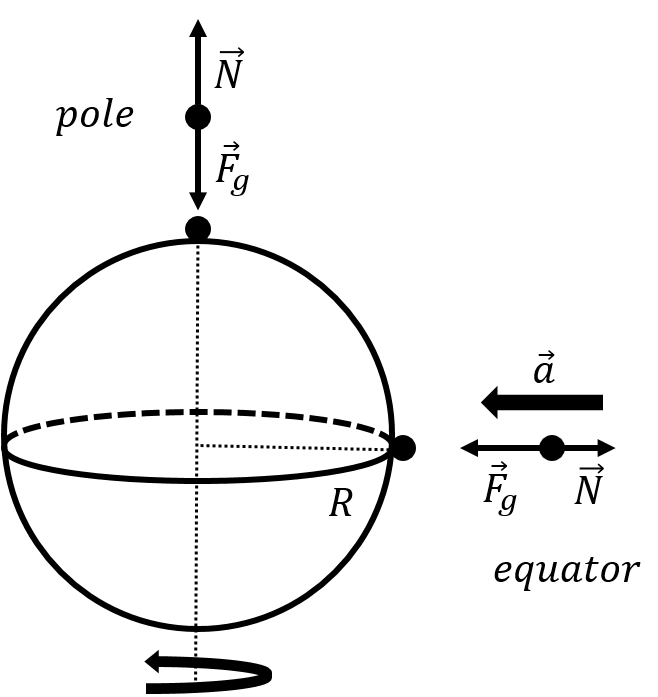
\includegraphics[width=0.4\linewidth]{files/apparentweight-1bb883d1a3842318caf1d98114381ea2.png}
\caption[]{The apparent weight, given by the normal force, is different at the Earth's equator because a person's acceleration is non-zero as they rotate with the Earth.}
\label{fig:gravity:apparentweight}
\end{figure}

Consider, instead, a person standing on a spring scale at the equator (Figure~\ref{fig:gravity:apparentweight}). That person is accelerating because they are undergoing uniform circular motion as they rotate along with the Earth. Again, the only forces acting on the person are their weight and the normal force exerted by the scale. The sum of the forces must now be equal to the person's mass, $m$, times the radial acceleration, $a_r$, that is necessary for them to follow the surface of the Earth as the Earth rotates about its axis. Newton's Second Law allows us to find the magnitude of the normal force acting on the person:
\begin{equation}
\sum F &= F_g-N=ma_r=m\frac{v^2}{R}\\
\therefore N &= F_g - m\frac{v^2}{R}\\
&=G\frac{Mm}{R^2} -  m\frac{v^2}{R}\\
&=m\left(G\frac{M}{R^2} - \frac{v^2}{R}  \right)\\
&=m\left(g - \frac{v^2}{R}  \right)
\end{equation}
where $M$ is the mass of the Earth, $R$ is the radius of the Earth, and $v$ is the speed at the surface of the Earth due to the Earth's rotation.  In the last line, we used the result from Example~9.3 where we determined the value of $g$ in terms of the mass and radius of the Earth.

We see that the normal force is reduced compared to what it would be if the Earth were not rotating ($v=0$) or if one is standing at one of the poles. Your apparent weight, which you can measure by standing on a spring scale, is thus smaller at the equator than it is at the poles. The quantity in parenthesis can be thought of as a modified or ``effective'' value of $g$ at the equator.

\begin{framed}
\textbf{Checkpoint}\\
What is the effective value of $g$ at the equator?

\begin{enumerate}
\item $9.80 {\rm m/s^2}$
\item $9.78 {\rm m/s^2}$
\item $9.70 {\rm m/s^2}$
\item $9.51 {\rm m/s^2}$
\end{enumerate}

\begin{framed}
\textbf{Answer}\\
\begin{enumerate}[resume]
\item
\end{enumerate}
\end{framed}
\end{framed}

If you are circling the Earth a distance $R$ from the centre of the Earth at a constant speed $v$, it is possible for your apparent weight to be zero. Imagine standing on a scale in an aircraft that is circling the Earth and measuring your apparent weight with the spring scale. As the speed of the aircraft increases, your apparent weight, $N$, decreases according to the formula that we just found:
\begin{equation}
N=m\left(G\frac{M}{R^2} - \frac{v^2}{R}  \right)
\end{equation}
At a certain speed, $v$, your apparent weight is zero and you feel weightless:
\begin{equation}
G\frac{M}{R^2} &= \frac{v^2}{R}\\
\therefore v&= \sqrt{G\frac{M}{R} }
\end{equation}
This speed corresponds to a centripetal acceleration that is exactly equal to that due to gravity. This makes sense, since gravity is the only force that is acting on you (the normal force is now zero), which is exactly what we call being in orbit.

Earth's rotation has some interesting consequences for stationary objects. At any position on Earth that is not at the equator or the poles, the sum of the forces on any stationary object (meaning stationary relative to the Earth's surface) cannot be zero. This is because the object must rotate along with the Earth, so the net force on the object must point toward the centre of the circle about which that location on Earth is rotating.

Take, for example, a plumb line, which consists of a mass hanging from a string. The two forces acting on the mass are gravity and tension. The force of gravity must point towards the centre of the Earth. We would expect that the force of tension, and therefore the string, would point directly away from the centre of the Earth. However, we find that if the plumb line is located at some angle $\theta$ from the equator (but not at the equator or poles), as in Figure~\ref{fig:gravity:apparentweight2}, then the string will point slightly away from the centre of the Earth.  In order for the mass to remain stationary relative to the ground, it must rotate along with the Earth (radius $R$) around a circle of radius $R\cos\theta$.   Thus, the tension from the string cannot point away from the centre of the Earth, because the net force must point towards the centre of the circle of radius $R\cos\theta$.

\begin{figure}[!htbp]
\centering
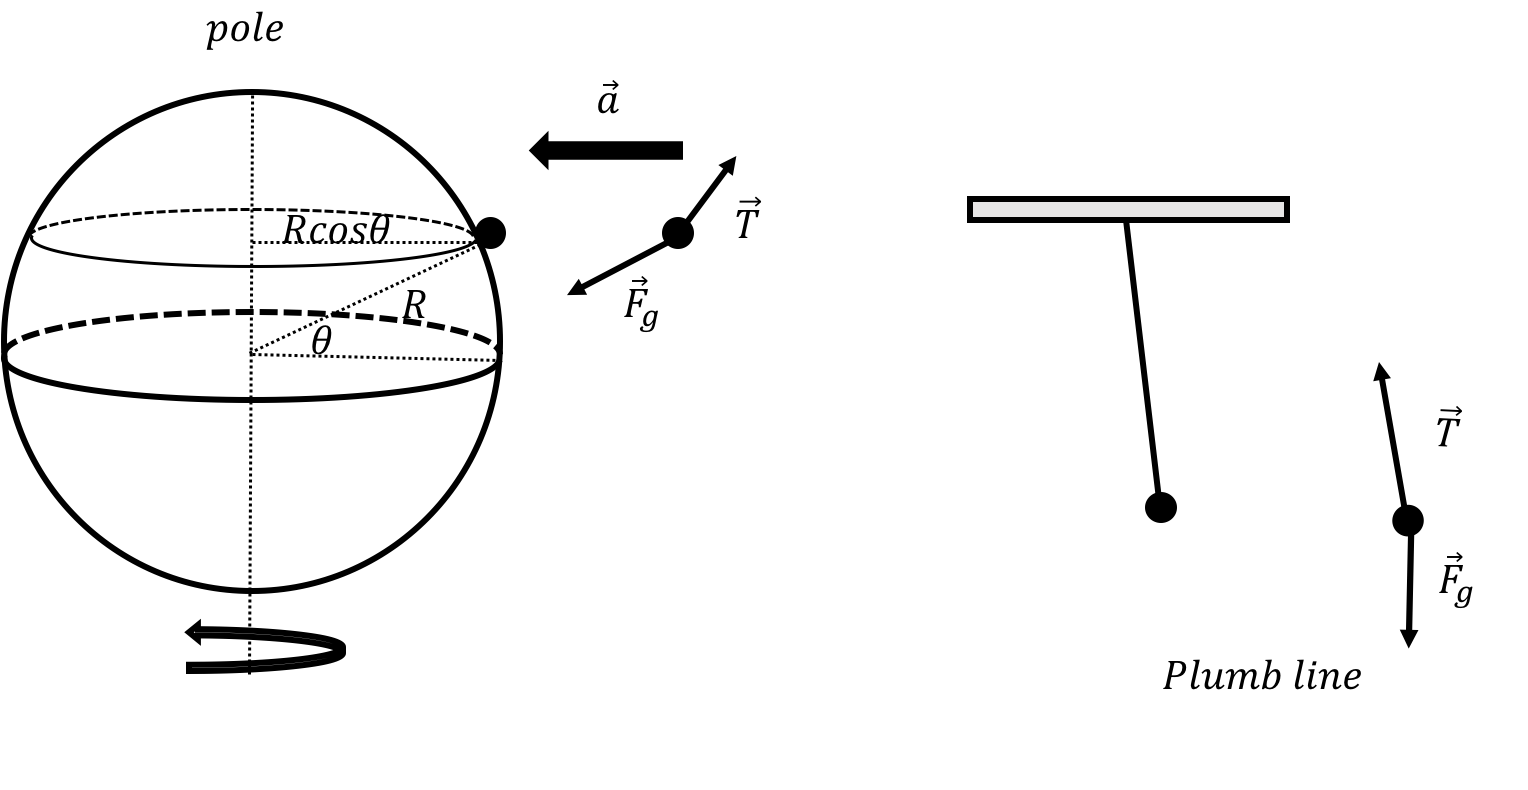
\includegraphics[width=0.8\linewidth]{files/apparentweight2-c000843b2433473a77dfad5122536b17.png}
\caption[]{Away from the equator and poles, a plumb line (right) does not point towards the centre of the Earth, because the net force on the mass must provide the acceleration towards the centre of the circle (of radius $R\cos\theta$) about which the plumb line rotates due to the Earth's rotation. Note that the deflection of the plumb line is highly exaggerated.}
\label{fig:gravity:apparentweight2}
\end{figure}

\begin{framed}
\textbf{Checkpoint}\\
You cut the string of the plumb line. Where does the mass land relative to its initial latitude (the angle $\theta$ in Figure~\ref{fig:gravity:apparentweight2})?

\begin{enumerate}
\item At the same latitude.
\item Closer to the nearest pole.
\item Closer to the equator.
\end{enumerate}

\begin{framed}
\textbf{Answer}\\
\begin{enumerate}
\item
\end{enumerate}
\end{framed}
\end{framed}

\paragraph{The gravitational field}

The gravitational force exerted on a mass $m$ by a mass $M$ can be written as:
\begin{equation}
\vec F(\vec r) = -G\frac{Mm}{r^2}\hat r
\end{equation}
if we define a coordinate system with the origin located at the centre of mass $M$ so that $\vec r$ is the position of $m$ relative to $M$. We can define the ``gravitational field'', $\vec g(\vec r)$, at position, $\vec r$, due to the presence of mass $M$ as the gravitational force per unit mass exerted by $M$:
\begin{equation}
\boxed{\vec g(\vec r) = \frac{\vec F(\vec r)}{m} =  - \frac{GM}{r^2}\hat r}
\end{equation}
The word ``field'' is just a mathematical term for a function that depends on position. Since $\vec g(\vec r)$ is a vector, we would refer to it as a ``vector field''.

Defining the gravitational field makes it easy to calculate the force of gravity from $M$ on any mass $m$:
\begin{equation}
\vec F_g = m\vec g(\vec r)
\end{equation}

At the surface of the Earth, the magnitude of the gravitational field is given by:
\begin{equation}
g(R_\oplus)=\frac{GM}{R_\oplus^2}=9.81 {\rm N/kg}
\end{equation}
where $R_\oplus$ is the radius of the Earth. Of course, this also corresponds to the acceleration of objects in free-fall near the surface of the Earth, which we can find from Newton's Second Law:
\begin{equation}
\sum \vec F &= \vec F_g = m\vec a\\
m\vec g(R_\oplus)&= m\vec a\\
\therefore \vec a &= \vec g(R_\oplus)
\end{equation}
but we see here why it more precise to refer to $g$ as the ``magnitude of the gravitational field at the surface of the Earth'' rather than ``the acceleration due to Earth's gravity''. It is also worth noting that the two are only equal if the gravitational mass (on the left of the equation in the second line) is the same as the inertial mass (on the right of the equation). The gravitational mass is the mass that appears in the gravitational force defined by Newton, whereas the inertial mass is the mass that appears with the acceleration in Newton's Second Law.

\begin{framed}
\textbf{Checkpoint}\\
Two small objects with different masses, $m_1$ and $m_2$, are located a distance $r$ from a nearby star. What can you say about the magnitude of the gravitational field and the magnitude of the gravitational force on $m_1$ and $m_2$?\}

\begin{enumerate}
\item The field is different and the forces are different.
\item The field is different but the forces are the same.
\item The field is the same but the forces are different.
\item The field is the same and the forces are the same.
\end{enumerate}

\begin{framed}
\textbf{Answer}\\
\begin{enumerate}[resume]
\item
\end{enumerate}
\end{framed}
\end{framed}

Suppose that there are two large mass bodies, $M_1$ and $M_2$, and a smaller mass body, $m$. We can calculate the net gravitational force on $m$ by summing the gravitational force vectors from $M_1$ and $M_2$ separately. If the gravitational fields from $M_1$ and $M_2$ are given by $\vec g_1(\vec r)$ and $\vec g_2(\vec r)$, respectively, then the total gravitational force on $m$ is given by:
\begin{equation}
\vec F &= m\vec g_1(\vec r) + m\vec g_2(\vec r)=m(\vec g_1(\vec r)+\vec g_2(\vec r))\\
&=m \vec g(\vec r)
\end{equation}
where we have introduced the total gravitational field:
\begin{equation}
\vec g(\vec r) = \vec g_1(\vec r)+\vec g_2(\vec r)
\end{equation}
In other words, if there are multiple bodies that result in a non-negligible force of gravity, we can calculate their gravitational fields independently and sum them together to define a net gravitational field, $\vec g(\vec r)$, that models the net force of gravity from all of the bodies. The net gravitational force on a new body of mass $m'$ is then simply given by $m'\vec g(\vec r)$, and we do not need to add any more vectors together. For example, when calculating the motion of satellites that can be influenced by the force of gravity from both the Earth and the Moon, we simply need to calculate the net gravitational field from the Earth and Moon, and the motion of any satellite can then be modelled using that net gravitational field.

\begin{framed}
\textbf{Checkpoint}\\
There are two planets with equal mass located a distance $d$ apart. Position $A$ is located midway between the two planets. Position $B$ is located a distance $d/2$ from one of the planets, in the position shown in Figure~\ref{fig:gravity:fieldAB}. How does the field at $A$ compare to the field at $B$

\begin{figure}[!htbp]
\centering
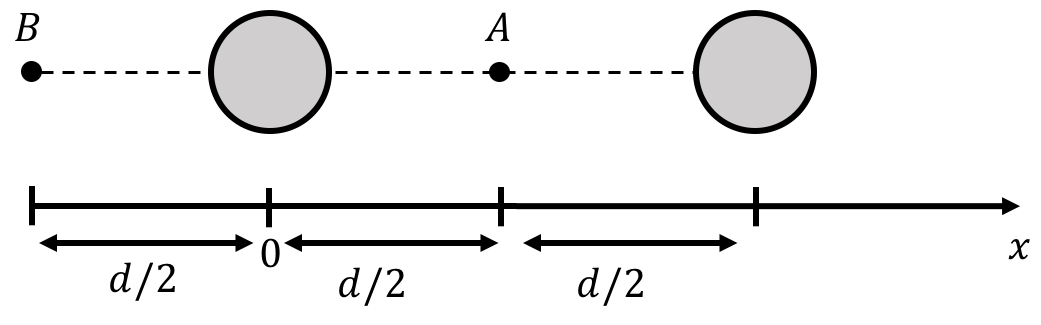
\includegraphics[width=0.6\linewidth]{files/fieldAB-8b5177e687c3f0a0914470d3ce9c2cde.png}
\caption[]{Two planets are a distance $d$ apart. We are considering the gravitational field at two positions, A and B, located near the planets.}
\label{fig:gravity:fieldAB}
\end{figure}

\begin{enumerate}
\item The magnitude of the field is the same at $A$ and $B$.
\item The magnitude of the field is greater at $A$ than at $B$.
\item The magnitude of the field is greater at $B$ than at $A$.
\end{enumerate}

\begin{framed}
\textbf{Answer}\\
\begin{enumerate}[resume]
\item
\end{enumerate}
\end{framed}
\end{framed}

\paragraph{Gauss's Law}\label{sec:gravity:gauss}

Newton's Universal Theory of Gravity postulates that the force of gravity between two bodies decreases as the squared of the distance between those two bodies. Using the terminology of a field, we would say that the strength of the gravitational field from an object decreases as the inverse of the square of the distance to that object. This is an example of a what we generally call an ``inverse-square law''. The electric force between two charges is also given by an inverse-square law, and we now understand that these forces behave as if they were ``transmitted'' by waves or particles.

If a force is given by an inverse-square law, then Gauss's law gives a way to determine the strength of the field that is associated with that force. In the case of gravity, Gauss's law states that:
\begin{equation}
\oint \vec g(\vec r) \cdot d\vec A = 4\pi G M^{enc}
\end{equation}
where the integral on the left is an integral over a ``closed surface'' that completely surrounds the mass for which we want to determine the gravitational field. To evaluate the integral, imagine taking a closed surface, $S$, that surrounds the mass. The vector $d\vec A$ is defined as the vector that goes with a small element of that surface and points outwards from the closed surface. The magnitude of the vector is equal to the area of that small surface ($dA$), as illustrated in Figure~\ref{fig:gravity:gauss}. You can then take the scalar product of $d\vec A$ with the gravitational field, $\vec g(\vec r)$, at that point on the surface. If you sum all of those scalar products, you get the value of the integral on the left. Gauss's law states that the value of that integral is equal $4 \pi G$ times the total mass that is enclosed by the surface.

\begin{framed}
\textbf{Olivia's Thoughts}\\
If you want to know if a surface is closed, ask yourself if you could put water inside the surface and not be worried about it spilling out. For example, if you put water in a sphere or a cube , the water would not spill out even if you shook it around, so they are closed surfaces. A flat square is an open surface because there is no ``inside'' to even put the water in.  A bowl is an open surface because, though you can put water in it, the water could spill out.
\end{framed}

We will go into more detail about Gauss's law when we cover electromagnetism, but it is worth seeing how to use it in a simple scenario. Figure~\ref{fig:gravity:gauss} shows a spherical body of mass $M$ and radius $R$ for which we would like to determine the value of the gravitational field at a distance $r$ from the centre of the body.

\begin{figure}[!htbp]
\centering
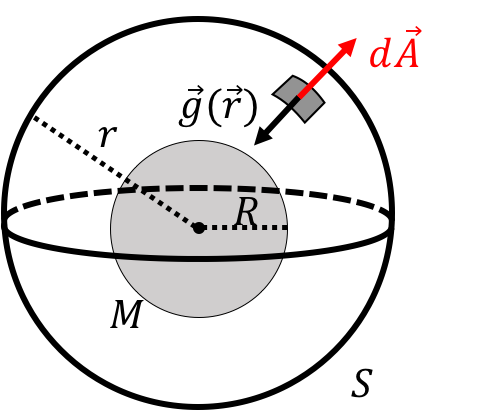
\includegraphics[width=0.3\linewidth]{files/gauss-532f5d1a8160ab32373485383e5e63f6.png}
\caption[]{Example of a spherical Gaussian surface, $S$, of radius $r$ centred about a body of mass $M$ and radius $R$. An element of the surface, $d\vec A$ is also shown along with the gravitational field, $\vec g(\vec r)$, at that point.}
\label{fig:gravity:gauss}
\end{figure}

To do so, we draw a ``Gaussian surface'', $S$, that is a sphere with a radius $r$, and centred about the body. At any point on the surface, the area element vector $d\vec A$ points away from the centre of the spherical surface. The gravitational field vector, $\vec g(\vec r)$ will always point towards the centre of the spherical surface, as illustrated. Furthermore, by symmetry, the magnitude of $\vec g(\vec r)$ is constant along the whole Gaussian surface. Thus, the scalar product $\vec g(\vec r) \cdot d\vec A= -g(r)dA$ everywhere along the surface (it is negative because the two vectors are anti-parallel). The integral is thus given by:
\begin{equation}
\oint \vec g(\vec r) \cdot d\vec A = -g(r)\oint dA
\end{equation}
where we factored $g(r)$ out of the integral, since the magnitude of $\vec g(\vec r)$ is constant for all of the area elements $dA$ on the sphere. Remember that an integral is a sum. The integral $\oint dA$ thus means ``sum all of the area elements $dA$ over the entire surface $S$''. Thus, the integral is the total area of the spherical surface $S$\footnote{The surface area of a sphere of radius $r$ is $4\pi r^2$.}:
\begin{equation}
\oint \vec g(\vec r) \cdot d\vec A = -g(r)\oint dA =-g(r)(4\pi r^2)
\end{equation}
Inserting this into Gauss's law, we find:
\begin{equation}
\oint \vec g(\vec r) \cdot d\vec A &= 4\pi G M^{enc}\\
-g(r)(4\pi r^2) &= 4\pi G M^{enc}\\
\therefore g(r) &= - \frac{GM}{r^2}
\end{equation}
where $M^{enc}=M$ is the total mass enclosed by the Gaussian surface (in this case, the entire mass $M$ is enclosed). This is of course the result that we expected and obtained earlier from Newton's formulation. Note that Gauss's law is only easy to use if the system is highly symmetric (e.g. spherically symmetric), and that it does not give the direction of the field vector, which must be obtained from symmetry arguments.

\begin{framed}
\textbf{Olivia's Thoughts}\\
Here's an analogy to describe Gauss's law for gravity: A famous celebrity is doing an event, and they attract a certain number of fans who want to get as close to the celebrity as possible. You put up a barricade around the celebrity. The gravitational field is represented by how crowded it is somewhere along the barricade. If a second celebrity is at the event, they will attract their own fans, so there will be more people around the barricade. The number of celebrities is kind of like the enclosed mass $M^{enc}$.

A photographer is coming to the event, and you told him to stand at some location that is a distance $r$ from the celebrities. The photographer wants to know how crowded it will be when he is standing behind the barricade at that location. Gauss's law gives us a way to figure this out. If you know which celebrities are at the event ($M^{enc}$), you can determine how many people will be there (this is like finding $4\pi GM^{enc}$). Then, if you can build a barricade such that the fans are evenly distributed around it, and you know how long that barricade is ($\oint dA$), you can easily calculate how crowded it will be at some point along the barricade (you can just divide the number of people by the length of the barricade).

The barricade represents our Gaussian surface and, like a Gaussian surface, it can be whatever shape we want as long as it encloses the celebrities and passes through the point we are interested in. If we want to make sure the people are spread out evenly, the shape of the barricade is going to depend on the specific case. Let's take the example of our single spherical body. This is analagous to having one celebrity at the event.

Figure~\ref{fig:gravity:barricadeanalogy} shows two possible barricades we could build. Although we can technically build the barricade on the left, it doesn't help us because the areas closer to the celebrity will be more crowded. Instead, we want to build the barricade on the right, which is a circle of radius $r$, because the fans are evenly spread out. This is why we use a spherical Gaussian surface when we're considering the field due to a spherical body - at any point a distance $r$ from the body, the field will be the same. (Note: Remember that, unlike the barricade, the Gaussian surface isn't a physical thing, so it won't affect the gravitational field. It is just a mathematical tool that allows us to take advantage of what the field already looks like.)

\begin{figure}[!htbp]
\centering
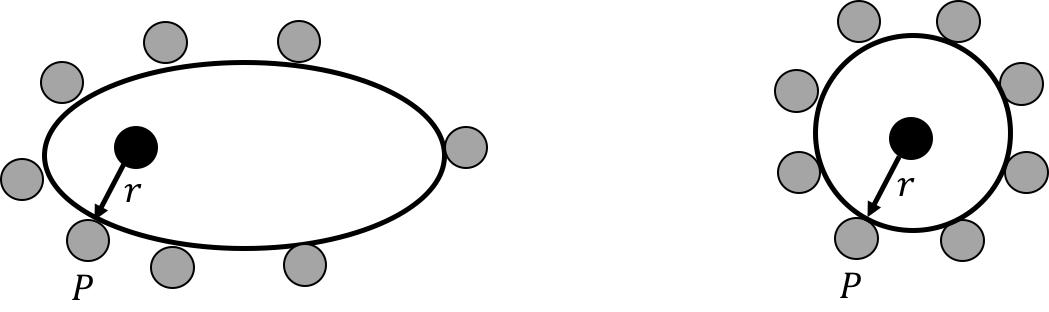
\includegraphics[width=0.7\linewidth]{files/barricadeanalogy-98ef92293c7c725259688fc9eacd1a31.png}
\caption[]{A celebrity (black dot) attracts fans (grey dots). A photographer (dot labelled ``P'') stands behind the barricade a distance $r$ away. This shows two possible barricades we could build around the celebrity. The density of the fans is not uniform for the barricade on the left, so we would not choose that shape to evaluate the Gaussian integral.}
\label{fig:gravity:barricadeanalogy}
\end{figure}
\end{framed}

We can also use Gauss's law to determine the gravitational field \textbf{inside} of the body of mass $M$ and radius $R$. This is illustrated in Figure~\ref{fig:gravity:gauss2}, which shows a spherical Gaussian surface of radius $r$ that is \textbf{inside} of the body of mass $M$.

\begin{figure}[!htbp]
\centering
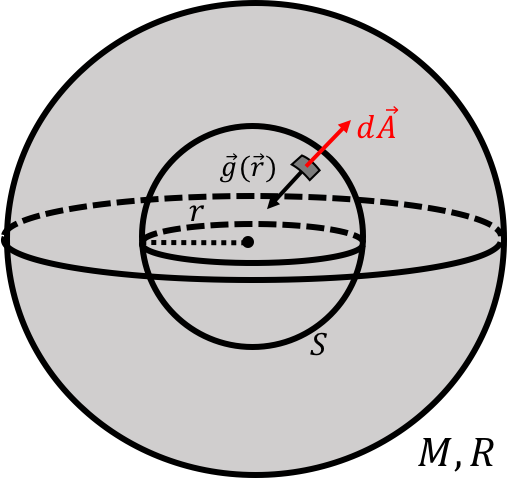
\includegraphics[width=0.3\linewidth]{files/gauss2-3bcc1d70b85158fced3e532072fa9bf9.png}
\caption[]{Example of a spherical Gaussian surface, $S$, of radius $r$ centred inside a body of mass $M$ and radius $R$.}
\label{fig:gravity:gauss2}
\end{figure}

The gravitational field inside of the body of mass $M$ is also symmetric
and  constant in magnitude across the whole surface, \%?
so that the integral is the same as before:
\begin{equation}
\oint \vec g(\vec r) \cdot d\vec A=-g(r)(4\pi r^2)
\end{equation}
However, in order to use Gauss's law, we need to determine the mass of the body that is enclosed within the spherical surface, which will be less than $M$. If we assume that the mass density, $\rho$, of the object is constant (the body is made of a uniform material), then the density is simply the mass of the object over its volume:
\begin{equation}
\rho = \frac{M}{\frac{4}{3}\pi R^3}
\end{equation}
The amount of mass enclosed by the spherical surface of radius $r$ is the density multiplied by the volume of a sphere of radius $r$:
\begin{equation}
M^{enc} = \rho \frac{4}{3}\pi r^3 = M\frac{r^3}{R^3}
\end{equation}
Applying Gauss's law, we can now find the magnitude of the gravitational field inside of the spherical body at a distance $r$ from the centre:
\begin{equation}
\oint \vec g(\vec r) \cdot d\vec A &= 4\pi G M^{enc}\\
-g(r)(4\pi r^2) &= 4\pi G M\frac{r^3}{R^3}\\
\therefore g(r) &= - \frac{G M}{R^3}r
\end{equation}
And we find that, inside a uniform spherical body of mass $M$, the gravitational field increases linearly with radius as one moves out from the centre. At the centre of the body, the gravitational field is zero.

\begin{framed}
\textbf{Checkpoint}\\
What can you say about the magnitude of the gravitational field inside a spherical \textbf{shell} of mass $M$?

\begin{enumerate}
\item It increases as you move out from the centre of the spherical shell.
\item It decreases as you move out from the centre of the spherical shell.
\item It is equal to zero.
\item It is nonzero and constant in magnitude.
\end{enumerate}

\begin{framed}
\textbf{Answer}\\
\begin{enumerate}[resume]
\item
\end{enumerate}
\end{framed}
\end{framed}

\subsubsection{Gravitational potential energy}\label{sec:gravity:potentialenergy}

Consider a large spherical body of mass $M$ with a coordinate system whose origin coincides with the centre of the spherical body (for example, the large body could be the Earth). The force, $\vec F(\vec r)$ on a body of mass $m$ (for example, a satellite), located at a position $\vec r$ is then given by:
\begin{equation}
\vec F(\vec r) = - G\frac{Mm}{r^2}\hat r=- G\frac{Mm}{r^3}\vec r
\end{equation}
where in the second equality, we use the fact that the unit vector in the direction of $\vec r$ is simply the vector $\vec r$ divided by its magnitude. We can write the force out in Cartesian coordinates:
\begin{equation}
\vec r &= x\hat x + y \hat y + z\hat z\\
r &= \sqrt{x^2+y^2+z^2} =(x^2+y^2+z^2)^\frac{1}{2} \\
\therefore \vec F(x,y,z) &= - G\frac{Mm}{(x^2+y^2+z^2)^\frac{3}{2} }(x\hat x + y \hat y + z\hat z)
\end{equation}
Mathematically, this is equivalent to the force that we considered in Example~8.2 of Section~\ref{chapter:potentialecons}, which we showed was a conservative force. The force of gravity in Newton's theory is thus a conservative force, for which we can determine a potential energy function.

In order to determine the gravitational potential energy function for the mass $m$ in the presence of a mass $M$, we calculate the work done by the force of gravity on the mass $m$ over a path where the integral for work will be ``easy'' to evaluate, namely a straight line. Figure~\ref{fig:gravity:potential} shows such a path in the radial direction, $r$, over which it will be easy to calculate the work done by the force of gravity from mass $M$ when mass $m$ moves from being a distance $r_A$ to a distance $r_B$ from the centre of mass $M$.

\begin{figure}[!htbp]
\centering
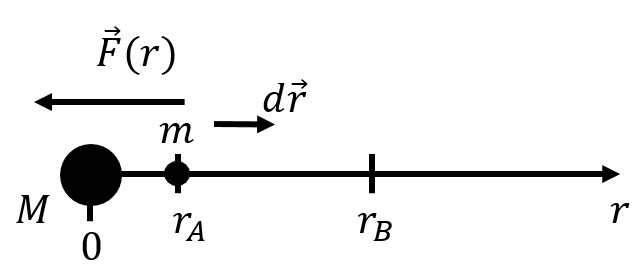
\includegraphics[width=0.5\linewidth]{files/potential-6cf2648356a2e39b57f407020da40b77.png}
\caption[]{Calculating the work done on a mass $m$ by the force of gravity exerted by mass $M$ when mass $m$ moves from a distance $r_A$ to a distance $r_B$ from the centre of mass $M$.}
\label{fig:gravity:potential}
\end{figure}

The work done by the force of gravity on $m$ in going from $r_A$ to $r_B$ is given by:
\begin{equation}
W &= \int_{r_A}^{r_B}\vec F(r) \cdot d\vec r = \int_{r_A}^{r_B} \left(- G\frac{Mm}{r^2}\hat r \right)\cdot d\vec r =\int_{r_A}^{r_B} - G\frac{Mm}{r^2}dr\\
&=\left[G\frac{Mm}{r} \right]_{r_A}^{r_B} =G\frac{Mm}{r_B} - G\frac{Mm}{r_A}
\end{equation}
The difference in potential energy in going from position $A$ to position $B$ is given by the negative of the work done by the force:
\begin{equation}
\Delta U = U(r_B) - U(r_A) = -W = G\frac{Mm}{r_A} - G\frac{Mm}{r_B}
\end{equation}
By inspection, we can identify the potential energy function for gravity:
\begin{equation}
\boxed{U(r) = -G\frac{Mm}{r} + C}
\end{equation}
which is determined only up to a constant, $C$.

A particularly useful choice of constant is $C=0$. This corresponds to choosing the potential energy to be zero only when $r$ goes to infinity. That is, the potential energy of mass $m$ is zero only when it is infinitely far away from mass $M$. The choice of constant $C$ corresponds to the (arbitrary) value of the potential energy when mass $m$ is infinitely far from mass $M$. When mass $m$ is not infinitely far away, it has \textbf{negative} potential energy (if $C=0$). This is not a problem! Remember, the only thing that is meaningful is a difference in potential energy, so the specific value of the potential energy has no meaning. The kinetic energy of an object, on the other hand, has to be positive.

Recall that if there are no other forces acting on an object, that object will move in such a way to reduce its potential energy. If the object of mass $m$ is located at some distance $r$ from the object of mass $M$, the force of gravity will attract $m$ so that $r$ decreases. As $r$ decreases in magnitude, the potential energy becomes more negative (larger in magnitude, but further away from zero), and the potential energy of $m$ will indeed decrease as it accelerates due to the force of gravity.

\paragraph{Mechanical energy with gravity}

Unless noted otherwise, we will continue our discussion of gravitational potential energy with the particular choice of constant $C=0$:
\begin{equation}
\boxed{U(r) = -G\frac{Mm}{r}}
\end{equation}
Furthermore, we will assume that $M$ is a large body, such as the Earth, which we can consider as fixed, and focus our discussion on describing the motion of mass $m$ (e.g. a satellite). If $M$ is much bigger than $m$, they will both experience a force of gravity from each other of the same magnitude (Newton's Third Law), but because $M$ is so much larger, its acceleration will be much smaller (Newton's Second Law). Thus, it is a good approximation to assume that $M$ is stationary and that only $m$ moves when $M>>m$.

We can define the total mechanical energy of mass $m$ when it has a speed $v$ (relative to $M$) and is located at a distance $r$ from the centre of mass $M$:
\begin{equation}
E = U + K = -G\frac{Mm}{r}+\frac{1}{2}mv^2
\end{equation}
where the kinetic energy term is always positive. If gravity is the only force exerted on mass $m$, then the mechanical energy, $E$, as defined above, will be a constant. The mechanical energy of an object can give us insight into the possible motion of the object.

Imagine launching a rocket straight upwards from the surface of the Earth; once all of the fuel has burnt up, the rocket's mechanical energy becomes constant as the rocket engine stops doing work on the rocket. As soon as the engine stops providing thrust, the rocket will start to slow down as the force of gravity attracts the rocket back to Earth. If the rocket is going fast enough, it will be able to completely escape the Earth's gravitational pull and travel to infinity (we assume that there are no other planets or the Sun, just the Earth exists!). If, on the other hand, the rocket's speed is too low, it will eventually stop and fall back to Earth. This is the same thing that happens to you when you try to jump vertically. If you could jump hard enough, you would be able to escape the Earth's gravitational pull!

In terms of mechanical energy, we can ask ourselves if the mechanical energy of the rocket is large enough to escape the Earth's gravitational pull. Specifically, we can ask ourselves what the value of the rocket's kinetic energy would be when it reaches infinity. The kinetic energy of the rocket is given by:
\begin{equation}
K = E - U
\end{equation}
If the rocket is infinitely far from the Earth, then its potential energy is zero, and the kinetic energy is equal to $E$.

If the mechanical energy, $E$, is negative, it is not possible for the rocket to ever make it to infinity because its kinetic energy would have to be negative. In other words, if the mechanical energy is negative, then the object of mass $m$ can never escape the gravitational pull of object $M$. We say that $m$ is ``gravitationally bound'' to $M$.

If the mechanical energy, $E$, is exactly zero, then the object's kinetic energy will become zero just as it reaches infinity. In other words, it will just barely be able to escape the gravitational pull from mass $M$. The condition for this to happen is:
\begin{equation}
E &= 0\\
K & = -U\\
\frac{1}{2}mv^2 &= G\frac{Mm}{r}\\
\therefore v_{esc} &= \sqrt{\frac{2GM}{r}}
\end{equation}
which we can interpret as a condition for the speed of the rocket. If at some distance $r$ from $M$, the rocket has the speed given by the condition above, then it will have enough kinetic energy to escape the gravitational pull of $M$. We call this speed the ``escape velocity''.

Finally, if the mechanical energy is greater than zero, then the rocket will have enough energy to escape the gravitational pull of $M$ and have a non-zero speed when it reaches infinity.

\begin{framed}
\textbf{Checkpoint}\\
What is the escape velocity from the surface of the Earth?

\begin{enumerate}
\item $4.29\times 10^{6} {\rm km/s}$
\item $1.25\times 10^{5} {\rm km/s}$
\item $11.2 {\rm km/s}$
\item $9.81 {\rm km/s}$
\end{enumerate}

\begin{framed}
\textbf{Answer}\\
\begin{enumerate}[resume]
\item
\end{enumerate}
\end{framed}
\end{framed}

\begin{framed}
\textbf{Example 9.4}\\
Show that an object of mass $m$ in a circular orbit of radius $r$ around a body of mass $M$ has half of the kinetic energy required to escape the gravitational pull of $M$.

\begin{framed}
\textbf{Solution}\\
The only force acting on the object is gravity, so it has a mechanical energy given by:
\begin{equation}
E&=U+K\\
E&=-G\frac{Mm}{r}+\frac{1}{2}mv^2
\end{equation}
In order for the object to just escape the gravitational pull of $M$, it's mechanical energy must be equal to zero:
\begin{equation}
E&=0\\
\therefore K_{esc}&=-U
\end{equation}
Since the object is in a circular orbit, we can use Newton's Second Law to find an expression for $v^2$:
\begin{equation}
F_{net}&=\frac{mv^2}{r}\\
\frac{GMm}{r^2}&=\frac{mv^2}{r}\\
\frac{GM}{r}&=v^2
\end{equation}
where in the second line we used the fact that $F_{net}$ is equal to the force of gravity exerted by $M$ on the object. The kinetic energy of the object is thus:
\begin{equation}
K&=\frac{1}{2}mv^2\\
K&=\frac{1}{2}\frac{GMm}{r}
\end{equation}
You will notice that this is very similar to our expression for $U$. In fact, we have:
\begin{equation}
K&=-\frac{1}{2}U\\
\therefore K&=\frac{1}{2}K_{esc}
\end{equation}
\textbf{Note:} We can also see that the velocity of an object in a circular orbit is equal to $\sqrt{GM/r}$, which is half the escape velocity, $v_{esc}=\sqrt{2GM/r}$
\end{framed}
\end{framed}

\subparagraph{Types of orbits}

The mechanical energy of a body of mass $m$ determines whether it is gravitationally bound to (i.e. cannot escape) the body of mass $M$. The path (orbit) that $m$ will take depends on its velocity with respect to $M$. Clearly, if the velocity of $m$ is directed at the centre of $M$, then $m$ will just collide with $M$. In all other cases, the orbit that $m$ will take depends on the mechanical energy of $m$ as well as the speed of $m$ at the point of closest approach to $M$ (see Figure~\ref{fig:gravity:conical}). The velocity of $m$ at the point of closest approach will always be perpendicular to the line joining the centres of $m$ and $M$. The different possible orbits are:

\begin{enumerate}
\item A \textbf{circular orbit} of radius $R$ (where $R$ is the distance of closest approach) if the \textbf{mechanical energy is negative} (i.e. it is bound) and the speed is exactly equal to the value necessary for the gravitational force to provide the required centripetal acceleration for uniform circular motion:
\end{enumerate}
\begin{equation}
\sum F = G\frac{Mm}{R^2} &= m\frac{v^2}{R}\\\therefore v_{circ}=\sqrt{\frac{GM}{R}}
\end{equation}
\begin{enumerate}[resume]
\item An \textbf{elliptical orbit} if the \textbf{mechanical energy is negative} and the speed at the point of closest approach is different than that required for a circular orbit.
\item A \textbf{parabolic orbit} if the \textbf{mechanical energy is exactly zero}.
\item A \textbf{hyperbolic orbit} if the \textbf{mechanical energy is bigger than zero}.
\end{enumerate}

The possible orbits are illustrated in Figure~\ref{fig:gravity:conical}, and are curves in the family of ``conic sections'', as they can be found by the intersection of a plane and a cone. All conic sections have at least one ``focus'' point (ellipses have two) that corresponds to the location of $M$.

\begin{figure}[!htbp]
\centering
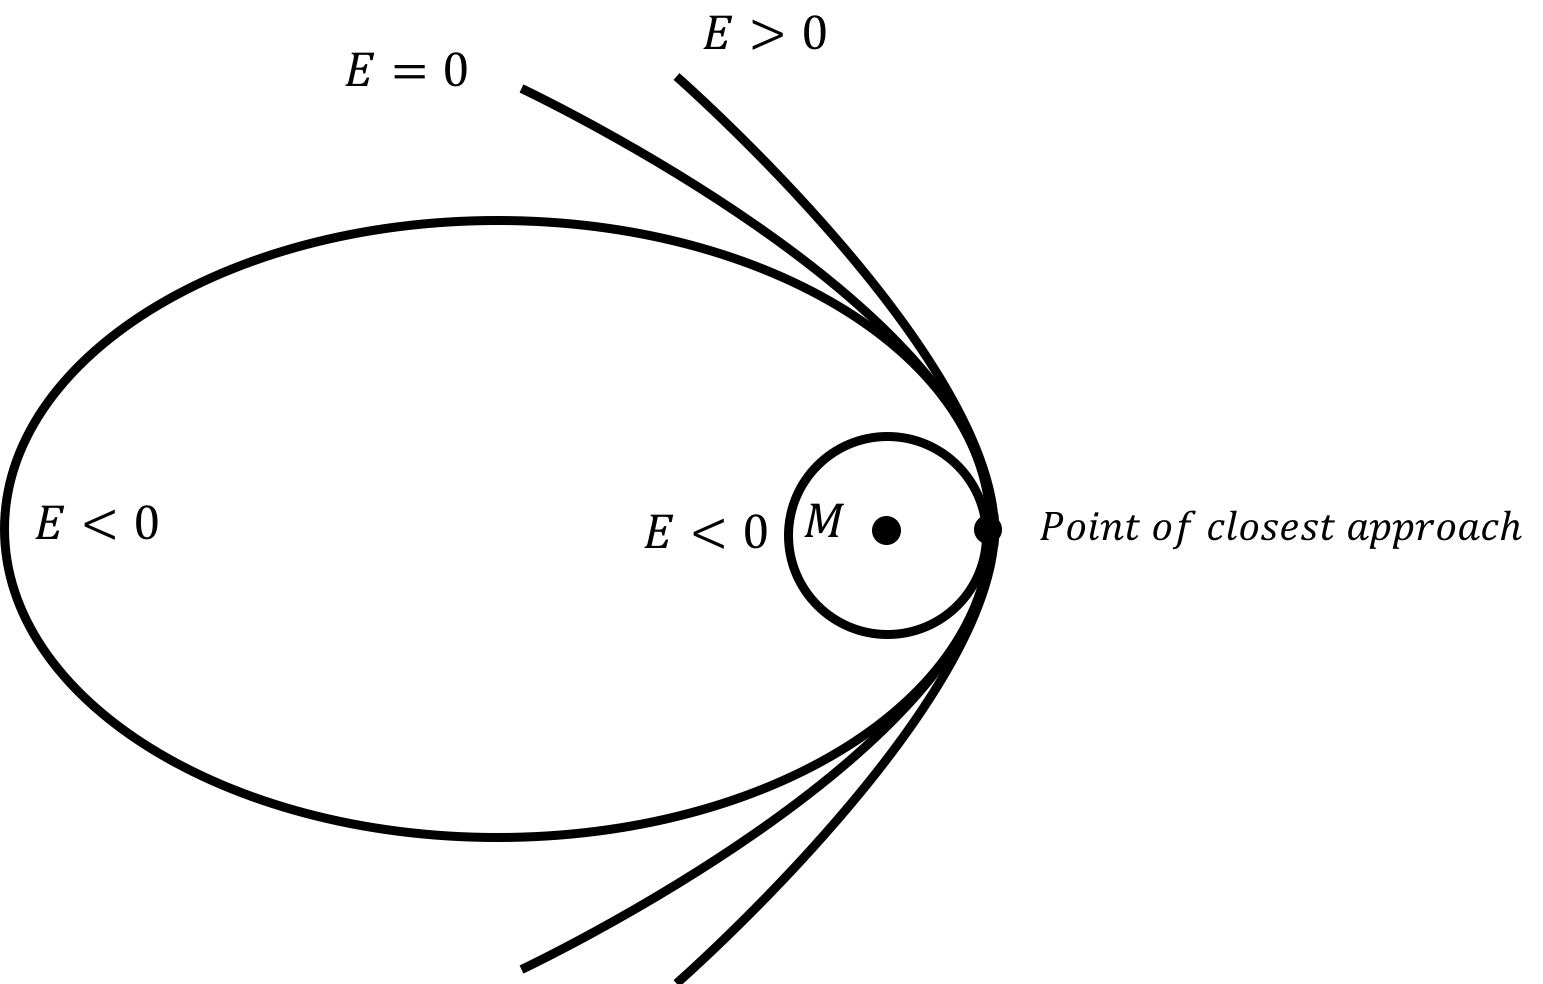
\includegraphics[width=0.7\linewidth]{files/conical-4e29b968e370c802d0ed276493194a28.png}
\caption[]{The different possible orbits of $m$ due to the gravitational force of $M$ depend on the mechanical energy, $E$, of $m$. The orbits are drawn in a frame of reference where $M$ is at rest.}
\label{fig:gravity:conical}
\end{figure}

\subsubsection{Einstein's Theory of General Relativity}

Newton's Universal Theory of Gravity was extremely successful at describing the motion of planets in the solar system, and allowed for high precision astronomy. For example, precision measurements of  Uranus's orbit showed that it appeared to be inconsistent with Newton's theory, unless the gravitational influence of another planet was included in the model. This led to the discovery of the planet Neptune.

However, some issues with Newton's theory were uncovered. The orbit of Mercury was shown to be different than what Newton's theory could describe, but searches for another planet (Vulcan) were unsuccessful. In addition, Albert Einstein's theory of Special Relativity, published in 1905, was found to be incompatible with Newton's theory of gravity. One of the consequences of Special Relativity is that nothing can propagate faster than the speed of light. Newton's Universal Theory of Gravity implies that the gravitational force is transmitted instantaneously. In Newton's theory, if the Sun suddenly disappeared, Earth would immediately ``fall out'' of its orbit, and we would immediately know that the Sun has disappeared. This would violate Special Relativity because there cannot be a mechanism that would allow us to know that the Sun has disappeared faster than it would take light to propagate from the Sun. In other words, for the $8 {\rm min}$ that are required for light to travel from the Sun to the Earth, we cannot know that the Sun has disappeared: only when we literally see the Sun disappear would the Earth be ``allowed'' to fall out of its orbit.

Einstein's Theory of General Relativity is a theory developed by Einstein in order to describe gravity in a way that is consistent with Special Relativity and the propagation of light. Einstein was famous for his ``thought experiments,'' which allow us to think about some of the implications of a theory, even if the experiments would be very difficult to carry out in practice. One such thought experiment is to consider what someone would observe in an accelerating frame of reference.

Consider an observer in an elevator, as illustrated in Figure~\ref{fig:gravity:elevator}. If the elevator is stationary at the surface of the Earth (left panel), and the observer is standing on a scale, they could measure their weight, $mg$, on the scale. The two forces on the observer are their weight and the normal force, which would be equal in magnitude since the observer is not accelerating. The normal force, read out by the scale, would thus correspond to their weight. To be more precise, the normal force would be equal to $m_Gg$, where $m_G$ is the gravitational mass of the observer (that mass which is related to the force of gravity experienced by a mass).

If the elevator was instead placed in empty space, and the elevator was accelerating upwards with an acceleration of $g$ (right panel), the observer would still be able to measure their weight by stepping on the scale. The only force on the observer is the normal force from the scale, which must be equal to its mass times their acceleration $N=m_Ia=m_Ig$, since the observer is accelerating with the elevator. In this case, it is the inertial mass of the observer, $m_I$, that comes into play, so the normal force read on the scale is $m_Ig$.

\begin{figure}[!htbp]
\centering
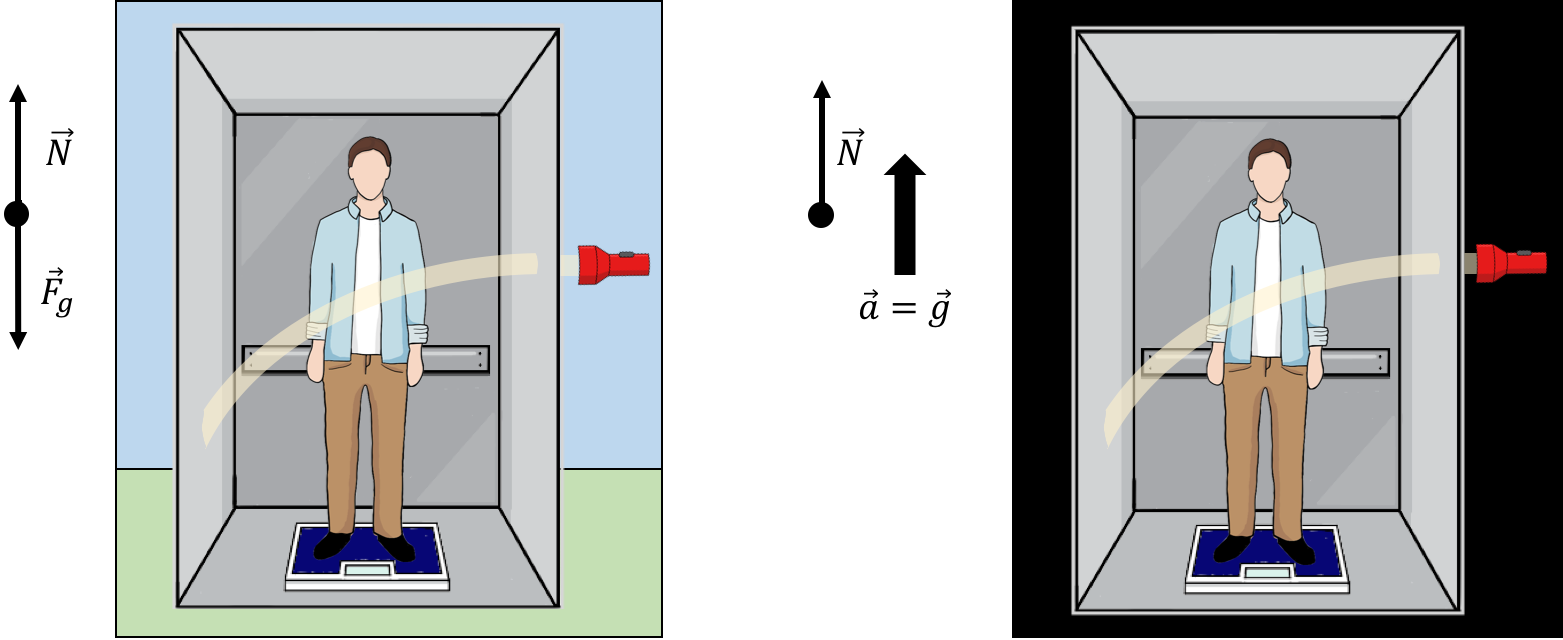
\includegraphics[width=0.8\linewidth]{files/elevator-cb051ec5733dec3aa2b4fdbfb11190a9.png}
\caption[]{Left: A person standing on a scale in an elevator at rest at the surface of the Earth. Right: A person in an elevator that is accelerating in empty space with the same acceleration as that due to gravity at the Earth's surface. The curvature of the light beam is exaggerated.}
\label{fig:gravity:elevator}
\end{figure}

Einstein postulated that it would be impossible for the observer to distinguish whether they are at rest on the surface of the Earth, or in empty space accelerating with an acceleration of $g$. In other words, he postulated that the inertial and gravitational masses are exactly equivalent. This is what is called the ``Equivalence Principle''.

This simple statement has dramatic implications. Special Relativity requires that light will travel in a straight line in empty space. If a beam of light enters and then exits the elevator, the observer on Earth and the one accelerating in empty space must observe the same thing, since they cannot distinguish between being on Earth or accelerating in space. The observer in space, who is accelerating, will observe that the beam of light bends as it crosses the elevator (the beam travels in a straight line as observed in an inertial reference frame, so the person in the accelerating elevator would see it follow a parabolic path). The observer on Earth must thus observe the same thing, namely that light will follow a curved path in the presence of a gravitational field.

But...light must travel in a straight line in empty space. That means that if the path of a beam of light is curved near Earth, it must be because space itself is curved in the presence of a gravitational field! In other words, Einstein's Theory of General Relativity describes how the presence of mass (or energy) results in a curvature of space (and time).

Imagine a ladybug on the side of a basketball. If the ladybug starts moving in what it believes to be a straight line, it will actually move in a curved path along the surface of the ball, as in Figure~\ref{fig:gravity:ladybug}. This is like the curved path of light that we observe. If we didn't know the ball was there, we would just think that the bug was moving along a curved path. In the same way, if an observer is not aware of the curvature of spacetime, it appears that light follows a curved path.

\begin{figure}[!htbp]
\centering
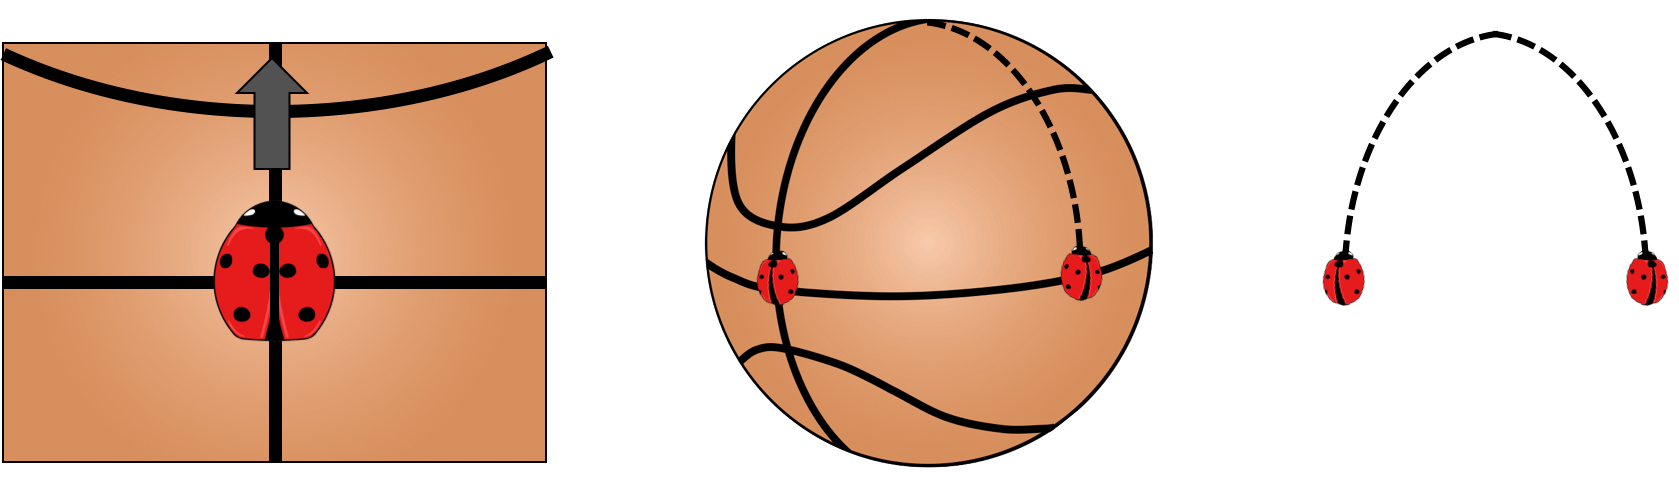
\includegraphics[width=0.8\linewidth]{files/ladybuganalogy-ceee73126e2939c41982b3bdb610b1d2.png}
\caption[]{Left: A ladybug perceives itself to be moving in a straight line. Center: The basketball is curved, so the ladybugs follow curved paths. Right: What an observer would see if they didn't know the basketball was there.}
\label{fig:gravity:ladybug}
\end{figure}

Now imagine there's a second ladybug. Both bugs start at the middle of the ball and start moving towards the top of the ball in what they think is a straight line (as shown in the center panel of Figure~\ref{fig:gravity:ladybug}). When the bugs start moving, they are parallel to each other, so if the ball was not curved, the ladybugs would never meet. However, because it is curved, the ladybugs will eventually cross paths. If you were not aware that the ball was there, you would have to conclude that there was some force attracting the bugs to each other, just like if you were unaware that spacetime was curved, you would conclude that massive bodies moving towards each other are attracted by a gravitational force.

Objects that are moving in a gravitational field are actually following Newton's First Law (they are moving at constant velocity in a straight line and no force is exerted on them). It is strange and unexpected, but high precision measurements confirm that this correctly describes everything that we have measured!

Einstein's theory was able to describe the orbit of Mercury, and the prediction that gravity leads to light following a curved path was confirmed by Eddington within five years of Einstein's theory being published. Another implication of the theory is that time goes by slower in the presence of a gravitational field. Clocks on Earth run slower than clocks in orbit (where the gravitational field is weaker). This effect is taken into account when using GPS to determine your position on Earth, since this is based on comparing the time that it takes signals to arrive to your position on Earth from different satellites. This is also somewhat reasonably well described in the movie ``Interstallar'', where time is seen to pass much slower for a set of astronauts in the vicinity of a black hole, where the gravitational field is strong.

\subsubsection{Summary}

Kepler was the first to synthesize a large amount of data to quantitatively describe gravity with his three laws:

\begin{enumerate}
\item The path of a planet around the Sun is described by an ellipse with the Sun at once of its foci.
\item Planets move in such a way that the area swept by a line connecting the planet and the Sun in a given period of time is constant, independent of the location of the planet.
\item The ratio between the orbital periods, $T$, squared of two planets is equal to the ratio of the semi-major axes, $s$, of their orbits cubed:
\end{enumerate}
\begin{equation}
\left(\frac{T_1}{T_2}\right)^2=\left(\frac{s_1}{s_2}\right)^3
\end{equation}

Newton described the attractive force of gravity exerted between two bodies of mass $M_1$ and $M_2$ (which must be point masses) as:
\begin{equation}
\vec F_{12}=-G\frac{M_1M_2}{r^2}\hat r_{21}
\end{equation}
where $\vec F_{12}$ is the force on body 1 from body 2, $r$ is the distance between the two bodies, and $\vec r_{21}$ is the vector from body 2 to body 1. The motion of a body under the influence of only this force will satisfy all of Kepler's Laws, if the body is gravitationally bound.

The gravitational field, $\vec g(\vec r)$, from a body of mass $M$, is defined as the gravitational force that another body would experience per unit mass:
\begin{equation}
\vec g(\vec r)=\frac{\vec F(\vec r)}{m}=-G\frac{M}{r^2}\hat r
\end{equation}
The field can be used to determine the corresponding gravitational force, $\vec F_g$, that a body of mass $m$ would experience if located at a position $\vec r$ relative to the body of mass $M$:
\begin{equation}
F_g = m \vec g(\vec r)
\end{equation}
When describing the motion of objects near the surface of the Earth, it is thus more precise to refer to $g=9.8 {\rm N/kg}$ as the magnitude of the Earth's gravitational field at the surface of the Earth, then to refer to $g=9.8 {\rm m/s^2}$ as the acceleration due to Earth's gravity. The two are only equal if gravitational mass (the $m$ in the above equation) and inertial mass (the $m$ in Newton's Second Law) are the same.

Gauss's law, which applies to all inverse-square force laws, can be used to determine the magnitude of the gravitational field from a body of mass $M$, even if it is not a point mass:
\begin{equation}
\oint \vec g(\vec r) \cdot d\vec A = 4\pi G M^{enc}
\end{equation}

Since the force described by Newton's theory is conservative, we can define a potential energy function. The gravitational potential energy of a mass $m$ located a distance $r$ away from a mass $M$ is:
\begin{equation}
U(r) = -G\frac{Mm}{r} + C
\end{equation}
A convenient choice of the constant is $C=0$, as this corresponds to the gravitational potential energy being equal to zero when $m$ is infinitely far away from $M$.

The mechanical energy, $E$, of an object of mass $m$ that is located at a distance $r$ from an object of mass $M$, if gravity is the only conservative force exerted on $m$, is given by:
\begin{equation}
E = K + U = \frac{1}{2}mv^2 - G\frac{Mm}{r}
\end{equation}
where we have explicitly chosen $C=0$, and $v$ is the speed of $m$ relative $M$ (considered to be at rest). Furthermore, if no non-conservative forces do work on the body of mass $m$, the mechanical energy, $E$, is constant.

If the mechanical energy of $m$ is negative, it is gravitationally bound to $M$. Depending on the mechanical energy of $m$ and its velocity at the point of closest approach to $M$, the orbit of $m$ will be described by one of four conic sections (circle, ellipse, parabola, hyperbola).

Einstein's Theory of General Relativity describes gravitation as the bending of space and time caused by the presence of mass and energy. In Einstein's theory, objects follow straight (inertial) paths and do not feel a force of gravity. The curvature of space is what results in their apparent motion not being a straight line. Einstein's theory is based on the Equivalence Principle (inertial and gravitational mass are exactly equal) and the properties of how light propagates according to the Theory of Special Relativity.
{\textbackslash}end\{chapterSummary\}

\begin{framed}
\textbf{Important Equations}\\
\textbf{Kepler's Third Law:}
\begin{equation}
\left(\frac{T_1}{T_2}\right)^2=\left(\frac{s_1}{s_2}\right)^3
\end{equation}
\textbf{Gravitational force and{\textbackslash}~gravitational field:}
\begin{equation}
\vec F_{12}&=-G\frac{M_1M_2}{r^2}\hat r_{21}\\
\vec g(\vec r)&=-G\frac{M}{r^2}\hat r\\
F_g &= m \vec g(\vec r)
\end{equation}

\textbf{Gauss's Law:}
\begin{equation}
\oint \vec g(\vec r) \cdot d\vec A = 4\pi G M^{enc}
\end{equation}
\textbf{Gravitational potential energy{\textbackslash}~and mechanical energy:}
\begin{equation}
U(r) = -G\frac{Mm}{r} + C\\
E = K + U = \frac{1}{2}mv^2 - G\frac{Mm}{r}
\end{equation}
\end{framed}

\subsubsection{Thinking about the material}

\begin{framed}
\textbf{Reflect and research}\\
\begin{itemize}
\item When you look at the night sky, how can you tell the difference between a planet and a star?
\item What was the relationship between Tycho Brahe and Johannes Kepler?
\item How did Tycho Brahe collect all the data that Kepler used?
\item How much time elapsed between Kepler publishing his laws and Newton publishing his Universal Theory of Gravity?
\item What was Kepler's original intention when he synthesized Tycho Brahe's observations? What was he hoping to show?
\item What was Ptolemy's theory of gravity based upon?
\item Who was the first to suggest that planets revolved around the Sun instead of the Earth?
\item Explain how the force of gravity from the moon results in tides on both sides of the Earth.
\item Explain what an L1 Lagrange point is, and how it does not violate Kepler's Third Law.
\item How did Eddington confirm that light follows a curved path in a gravitational field?
\end{itemize}
\end{framed}

\begin{framed}
\textbf{To try in the lab}\\
\begin{itemize}
\item Theory project: Prove, based on Newton's Universal Theory of Gravity, that the motion of orbiting bodies is given by a conic section.
\item Write a computer simulation to plot the orbit of two bodies, and explore how the total mechanical energy of one object affects its motion. If the two bodies have the same mass, and both move, where is the focus of the conical section describing their respective paths?
\item Propose an experiment to model and map the position of a planet in the night sky.
\end{itemize}
\end{framed}

\subsubsection{Sample problems and solutions}

\paragraph{Problems}

\begin{framed}
\textbf{Problem 9.1}\\
Geosynchronous satellites are satellites that are placed in a circular orbit around the Earth in such a way that their orbital period is synchronized with the $24 {\rm h}$ rotation period of the Earth. The advantage of geosynchronous satellites is that they are always above the same point on Earth, which makes them useful for establishing communication networks. At what altitude must geosynchronous satellites be placed?
\end{framed}

\begin{framed}
\textbf{Problem 9.2}\\
How much energy must be expended in order to place a satellite of mass $m=1000 {\rm kg}$ in a geosynchronous circular orbit around the Earth, if the satellite is launched from the North Pole of the Earth? How much energy is this per kilogram of satellite placed in orbit?
\end{framed}

\begin{framed}
\textbf{Problem 9.3}\\
Find an expression for the gravitational field due to a thin uniform rod of mass $M$ at point $P$, which is a distance $h$ above the midsection of the rod (Figure~\ref{fig:gravity:rodfield}).

\begin{figure}[!htbp]
\centering
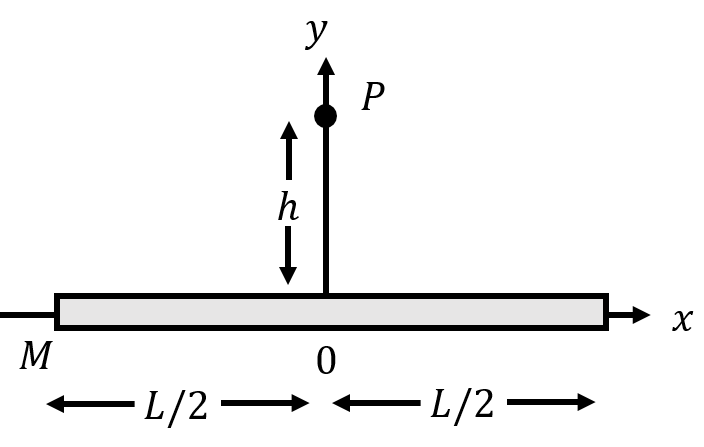
\includegraphics[width=0.5\linewidth]{files/rodfield-ac4b93fd8281a0c6f73aee0611dff3e2.png}
\caption[]{A thin rod of mass $M$ and length $L$ produces a gravitational field at a point $P$ located above the midsection of the rod.}
\label{fig:gravity:rodfield}
\end{figure}
\end{framed}

\paragraph{Solutions}

\begin{framed}
\textbf{Solution 9.1}\\
When a satellite orbits the Earth, the only force on the satellite is the force of gravity from the Earth. Since the satellite is in a circular orbit, that force of gravity must point towards the centre of the Earth in such a way that the satellite has the correct radial acceleration, $a_R$, to stay in uniform circular motion:
\begin{equation}
a_r=\frac{v^2}{R}
\end{equation}
where $v$ is the speed of the satellite, and $R$ is the distance between the satellite and the centre of the Earth (i.e. the centre of the circular orbit). The magnitude of the force of gravity on the satellite of mass $m$ is given by:
\begin{equation}
F = G\frac{Mm}{R^2}
\end{equation}
where $M$ is the mass of the Earth. Newton's Second Law applied to the satellite is:
\begin{equation}
\sum F_r = F &= ma_r\\
\therefore G\frac{Mm}{R^2}&=m\frac{v^2}{R}
\end{equation}
The speed of the satellite can be found from the fact that it must travel a distance of $2\pi R$ (the circumference of the orbit) in a period $T=24 {\rm h}$:
\begin{equation}
v=\frac{2\pi R}{T}
\end{equation}
which we can substitute into the equation from Newton's Second Law to find the distance $R$ (i.e. the radius of the circular orbit):
\begin{equation}
G\frac{Mm}{R^2}&=m\frac{v^2}{R}\\
G\frac{M}{R^2}&=\frac{(2\pi R)^2}{T^2R}\\ 
G\frac{M}{R^2}&=\frac{4\pi^2 R}{T^2}\\ 
\therefore R&=\sqrt[3]{G\frac{MT^2}{4\pi^2}}\\
&=\sqrt[3]{(6.67\times 10^{-11} {\rm Nm^2/kg^2})\frac{(5.97\times 10^{24} {\rm kg})(86400 {\rm s})^2}{4\pi^2}}\\
&=42.2\times 10^{6} {\rm m}
\end{equation}
which corresponds to the distance between the satellite and the centre of the Earth. To obtain the ``altitude'', $h$, namely the distance from the surface of the Earth to the satellite, we must subtract the radius of the Earth, $R_\oplus=6.371\times 10^{6} {\rm m}$ from this distance:
\begin{equation}
h = R-R_\oplus = 35.9\times 10^{6} {\rm m}
\end{equation}
Thus, geosynchronous satellites are located at an altitude of approximately $36000 {\rm km}$.

\textbf{Discussion}: Note that we could have also easily used Kepler's Third Law to determine the radius of the orbit, since we already know the period ($24 {\rm h}$), and we know the value of the constant for Kepler's Third Law from Example~9.2.
\end{framed}

\begin{framed}
\textbf{Solution 9.2}\\
We need to calculate how much work must be done for the satellite to go from being at rest at the surface of the Earth to being in a geosynchronous orbit. That work will be done by a non-conservative force (a rocket engine). The work done by the non-conservative force, $W$, is equal to the satellite's change in mechanical energy:
\begin{equation}
W = \Delta E = E_B -E_A
\end{equation}
The initial mechanical energy of the satellite, $E_A$, is given by its gravitational potential energy (it has no kinetic energy at the surface of the Earth when at the North Pole - on the equator, it would have kinetic energy due to the Earth's rotation):
\begin{equation}
E_A = K + U = 0 - G\frac{Mm}{R_\oplus}
\end{equation}
where $M=5.97\times 10^{24} {\rm kg}$ is the mass of the Earth, and $R_\oplus=6.731\times 10^{6} {\rm m}$ is the radius of the Earth.

In orbit, the energy of the rocket, $E_B$, is given by:
\begin{equation}
E_B = K + U = \frac{1}{2}mv^2 - G\frac{Mm}{R}
\end{equation}
where $R=42.2\times 10^{6} {\rm m}$ is the radius of the geosynchronous orbit (Problem~??) and $v$ is the speed of the satellite in orbit. The speed is given by:
\begin{equation}
v = \frac{2\pi R}{T}
\end{equation}
where $T=24 {\rm h}$ is the orbital period. The net work that must be done to place the satellite in orbit is thus given by:
\begin{equation}
W &= E_B - E_A = \frac{1}{2}mv^2 - G\frac{Mm}{R} - \left(- G\frac{Mm}{R_\oplus}\right)\\
&=\frac{1}{2}m\frac{4\pi^2 R^2}{T^2}+GMm\left(\frac{1}{R_\oplus}-\frac{1}{R}\right)\\
&=\frac{1}{2}(1000 {\rm kg})\frac{4\pi^2 (42.2\times 10^{6} {\rm m})^2}{(86400 {\rm s})^2}\\
&+(6.67\times 10^{-11} {\rm Nm^2/kg^2})(5.97\times 10^{24} {\rm kg})(1000 {\rm kg})\left(\frac{1}{(6.731\times 10^{6} {\rm m})}-\frac{1}{(42.2\times 10^{6} {\rm m})}\right)\\
&=5.78\times 10^{10} {\rm J}
\end{equation}
This corresponds to the energy that must be imparted to a $1000 {\rm kg}$ satellite for it to end up in a geosynchronous orbit. This corresponds to $5.78\times 10^{7} {\rm J/kg}$ as the energy required per kilogram of payload placed in geosynchronous orbit. Although we calculated work as if it were work done by a force, we can think of this work coming from stored chemical potential energy in the fuel of the rocket carrying the satellite.

\textbf{Discussion:} The energy that we found above is the minimum energy that one must provide to the satellite. In practice, in order to place a satellite in orbit, one will also need to provide enough energy to accelerate the rocket that carries the satellite up into orbit, which is typically much heavier than the satellite. If the satellite were instead launched from the equator of the Earth, the satellite would already have some initial kinetic energy due to the rotation of the Earth, and one would need to provide less energy to place it in orbit. This is the reason that most rockets are launched from near the equator (think French Guyana, Florida, Kazakhstan) in a direction that is roughly parallel with the Earth's rotation.
\end{framed}

\begin{framed}
\textbf{Solution 9.3}\\
We cannot use Gauss's law to determine the magnitude of the field because the gravitational field lacks symmetry (i.e. the field will be different at the ends of the rod than along the length of the rod). The gravitational field due to a body of mass $M$ is given by:
\begin{equation}
\vec g(\vec r)=-\frac{GM}{r^2}\hat{r}
\end{equation}

Our strategy will be to break the rod into very small segments of length $dx$. Each segment, of mass $dM$, will make a small contribution, $d\vec g$, to the gravitational field, as shown in Figure~\ref{fig:gravity:rodfieldsoln}. We will then take the sum of all these contributions to find the net field.

\begin{figure}[!htbp]
\centering
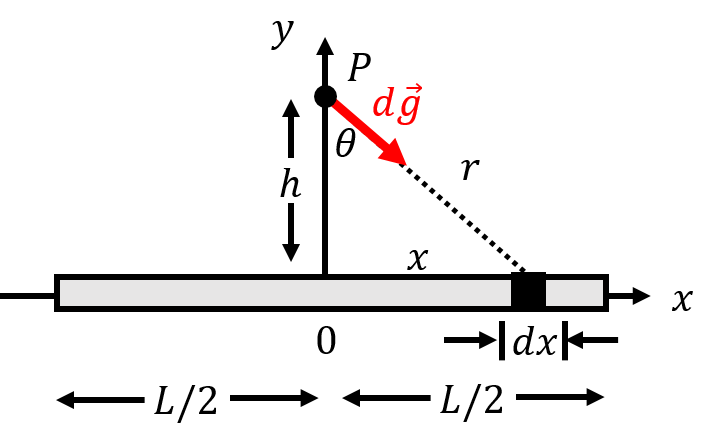
\includegraphics[width=0.5\linewidth]{files/rodfieldsoln-414a994c752a5af9ba19615e5119f9df.png}
\caption[]{A thin rod of mass $M$ and length $L$ produces a gravitational field at a point $P$ located above the midsection of the rod. Each segment of the rod $dx$ will contribute to the gravitational field.}
\label{fig:gravity:rodfieldsoln}
\end{figure}

The gravitational field due to each segment is given by:
\begin{equation}
d\vec g=-\frac{GdM}{r^2}\hat{r}
\end{equation}
The element of the field, $d\vec g$, will point in a different direction for each segment $dx$. You can conclude from Figure~\ref{fig:gravity:rodfieldsoln} that, due to symmetry, the $x$ components of the field from each segment will cancel out (for the segment $dx$ shown in the diagram, there will be an identical segment on the other side of the rod). The net field will point in the $-\hat{y}$ direction, so we are only interested in the vertical component of $d\vec g$. Using our diagram, this means that we want to find the magnitude of $dg\cos\theta$:
\begin{equation}
dg\cos\theta=\frac{G dM}{r^2}\cos\theta
\end{equation}
The magnitude of the gravitational field at point $P$ is thus given by:
\begin{equation}
g = \int dg\cos\theta =\int \frac{G dM}{r^2}\cos\theta
\end{equation}
The integral is written over $dM$, where both $r$, and $\theta$ are different for each different mass element, $dM$. We need to express any variable that changes for different mass elements in terms of a single variable of integration. We will choose $\theta$ as the variable of integration, and thus need to express $r$ and $dM$ in terms of $\theta$, $d\theta$, and other constants.

The distance, $r$, between $P$ and a mass element $dM$ located at angle $\theta$ is easily found to be:
\begin{equation}
r &= \frac{h}{\cos\theta}\\
\therefore \frac{1}{r^2} &= \frac{\cos^2\theta}{h^2}
\end{equation}

$dM$ can easily be expressed in term of $dx$ (the length of the mass element in the $x$ direction) and $\lambda$, the mass per unit length of the rod:
\begin{equation}
dM = \lambda dx = \frac{M}{L} dx
\end{equation}

We now need to express $dx$ in terms of $d\theta$. This can be found as follows, by first expressing $x$ in terms of $\theta$, and then taking the derivative of $x$ with respect to $\theta$
\begin{equation}
x &= h\tan\theta\\
\therefore \frac{dx}{d\theta}&=\frac{h}{\cos^2\theta}\\
\therefore dx  &= \frac{h}{\cos^2\theta} d\theta
\end{equation}
Now that we have found the small change in $x$ that results from a small change in $\theta$, we can write the mass element, $dM$, in terms of the $d\theta$:
\begin{equation}
dM = \frac{M}{L} dx = \frac{M}{L}  \frac{h}{\cos^2\theta} d\theta
\end{equation}
We can now write the integral in terms of $\theta$:
\begin{equation}
g = \int \frac{GdM}{r^2}\cos\theta&=G\int \frac{1}{r^2}\cos\theta dM\\
&=G\int \left( \frac{\cos^2\theta}{h^2} \right)\cos\theta \left(\frac{M}{L}  \frac{h}{\cos^2\theta}  \right)\\
&=\frac{GM}{Lh}\int\cos\theta d\theta
\end{equation}
Now that we have the integral over $\theta$, we need to set the limits to correspond to the values of $\theta$ at each end of the rod. The angle will have the same magnitude for each end of the rod, $\theta _0$, given by:
\begin{equation}
\sin\theta_0 =\frac{L}{2\sqrt{h^2 + \frac{L^2}{4}}}
\end{equation}
The magnitude of the field is thus given by:
\begin{equation}
g &=\frac{GM}{Lh}\int_{-\theta_0}^{\theta_0}\cos\theta d\theta\\
&= \frac{GM}{Lh} {\rm \left[n\theta\right]}_{-\theta_0}^{\theta_0}\\
&=\frac{2GM}{Lh} \sin\theta_0\\
&= \frac{2GM}{Lh} \frac{L}{2\sqrt{h^2 + \frac{L^2}{4}}}
\end{equation}
The gravitational field at point $P$ is thus given by:
\begin{equation}
\vec g =  -\frac{2GM}{Lh} \frac{L}{2\sqrt{h^2 + \frac{L^2}{4}}}\hat y
\end{equation}
\end{framed}